% answers.tex —— 2013 年·上海卷·理科 · 参考答案与详细解析片段
% 由 tools/generate_projects.py 依来源总账自 2013/2013_数学真题_上海理_试题.md + 2013/2013_数学真题_上海理_解析正文.md + 2013/2013_数学真题_上海理_答案要点.md 生成，勿手改（改源 MD 后重跑）


\begin{answer}
\gksolhead{1}{}

\textbf{题目}：

计算：$\lim\limits_{n\to\infty}\dfrac{n+20}{3n+13}=$\gkblank{}。

\Needspace{4\baselineskip}
\textbf{解析}
\Needspace{5\baselineskip}
分子、分母同除以 $n$：
\nopagebreak[4]
\[\lim_{n\to\infty}\frac{n+20}{3n+13}
=\lim_{n\to\infty}\frac{1+\dfrac{20}{n}}{3+\dfrac{13}{n}}
=\frac{1+0}{3+0}=\frac13.\]
故所求极限为 $\dfrac13$。

\gkanswer{答案：$\dfrac13$。分子、分母同除以 $n$，极限为 $\dfrac{1}{3}$。}

\end{answer}
\begin{answer}
\gksolhead{2}{}

\textbf{题目}：

设 $m\in\mathbf R$，$m^2+m-2+(m^2-1)\mathrm i$ 是纯虚数，其中 $\mathrm i$ 是虚数单位，则 $m=$\gkblank{}。

\Needspace{4\baselineskip}
\textbf{解析}
\Needspace{5\baselineskip}
设 $z=m^2+m-2+(m^2-1)\mathrm i$。$z$ 为纯虚数，当且仅当实部为零且虚部不为零：
\nopagebreak[4]
\[\begin{cases}
m^2+m-2=0,\\
m^2-1\neq0.
\end{cases}\]
\Needspace{5\baselineskip}
第一式因式分解得 $(m-1)(m+2)=0$，即 $m=1$ 或 $m=-2$。第二式给出 $m\neq\pm1$。因此 $m=1$ 被排除，只有
\nopagebreak[4]
\[m=-2.\]
此时 $z=(4-2-2)+(3)\mathrm i=3\mathrm i$，确为纯虚数。

\gkanswer{答案：$-2$。纯虚数要求 $m^2+m-2=0$ 且 $m^2-1\neq0$，故 $m=-2$。}

\end{answer}
\begin{answer}
\gksolhead{3}{}

\textbf{题目}：

若 $\begin{vmatrix}x^2&y^2\\-1&1\end{vmatrix}=\begin{vmatrix}x&x\\y&-y\end{vmatrix}$，则 $x+y=$\gkblank{}。

\Needspace{4\baselineskip}
\textbf{解析}
\Needspace{5\baselineskip}
按二阶行列式的定义展开：
\nopagebreak[4]
\[\begin{vmatrix}x^2&y^2\\-1&1\end{vmatrix}=x^2\cdot1-y^2\cdot(-1)=x^2+y^2,\]
\nopagebreak[4]
\[\begin{vmatrix}x&x\\y&-y\end{vmatrix}=x\cdot(-y)-x\cdot y=-2xy.\]
\Needspace{5\baselineskip}
由题设两式相等，得
\nopagebreak[4]
\[x^2+y^2=-2xy\iff x^2+2xy+y^2=0\iff (x+y)^2=0.\]
\Needspace{5\baselineskip}
故
\nopagebreak[4]
\[x+y=0.\]

\gkanswer{答案：$0$。左式为 $x^2+y^2$，右式为 $-2xy$，故 $(x+y)^2=0$。}

\end{answer}
\begin{answer}
\gksolhead{4}{}

\textbf{题目}：

已知 $\triangle ABC$ 的内角 $A$、$B$、$C$ 所对的边分别为 $a$、$b$、$c$。若 $3a^2+2ab+3b^2-3c^2=0$，则角 $C$ 的大小是\gkblank{}。（结果用反三角函数值表示）

\Needspace{4\baselineskip}
\textbf{解析}
\Needspace{5\baselineskip}
由 $3a^2+2ab+3b^2-3c^2=0$ 得
\nopagebreak[4]
\[c^2=a^2+\frac23ab+b^2.\]
\Needspace{5\baselineskip}
另一方面，余弦定理给出
\nopagebreak[4]
\[c^2=a^2+b^2-2ab\cos C.\]
\Needspace{5\baselineskip}
比较两式：
\nopagebreak[4]
\[-2ab\cos C=\frac23ab.\]
\Needspace{5\baselineskip}
因 $a,b>0$，可约去 $ab$，得
\nopagebreak[4]
\[\cos C=-\frac13.\]
\Needspace{5\baselineskip}
又 $C\in(0,\pi)$，故
\nopagebreak[4]
\[C=\arccos\left(-\frac13\right).\]

\gkanswer{答案：$\arccos\left(-\dfrac13\right)$。由余弦定理比较得 $\cos C=-\dfrac13$。}

\end{answer}
\begin{answer}
\gksolhead{5}{}

\textbf{题目}：

设常数 $a\in\mathbf R$。若 $\left(x^2+\dfrac ax\right)^5$ 的二项展开式中 $x^7$ 项的系数为 $-10$，则 $a=$\gkblank{}。

\Needspace{4\baselineskip}
\textbf{解析}
\Needspace{5\baselineskip}
二项展开式的通项为
\nopagebreak[4]
\[\mathrm C_5^k\left(x^2\right)^{5-k}\left(\frac ax\right)^k
=\mathrm C_5^k a^k x^{10-2k-k}
=\mathrm C_5^k a^k x^{10-3k},\qquad k=0,1,\cdots,5.\]
\Needspace{5\baselineskip}
令 $10-3k=7$，得 $k=1$。因此 $x^7$ 项的系数为
\nopagebreak[4]
\[\mathrm C_5^1a=5a.\]
\Needspace{5\baselineskip}
由 $5a=-10$ 得
\nopagebreak[4]
\[a=-2.\]
其余指数依次为 $10,7,4,1,-2,-5$，$x^7$ 项唯一，无遗漏。

\gkanswer{答案：$-2$。通项中 $x^7$ 对应 $k=1$，系数 $5a=-10$。}

\end{answer}
\begin{answer}
\gksolhead{6}{}

\textbf{题目}：

方程 $\dfrac{3}{3^x-1}+\dfrac13=3^{x-1}$ 的实数解为\gkblank{}。

\Needspace{4\baselineskip}
\textbf{解析}
\Needspace{5\baselineskip}
令 $t=3^x$，则 $t>0$ 且 $t\neq1$（分母 $3^x-1\neq0$）。原方程化为
\nopagebreak[4]
\[\frac{3}{t-1}+\frac13=\frac t3.\]
\Needspace{5\baselineskip}
两边乘以 $3(t-1)$：
\nopagebreak[4]
\[9+(t-1)=t(t-1),\]
\Needspace{5\baselineskip}
即
\nopagebreak[4]
\[t^2-2t-8=0.\]
\Needspace{5\baselineskip}
因式分解得 $(t-4)(t+2)=0$。由于 $t>0$，只有 $t=4$。于是
\nopagebreak[4]
\[3^x=4\Longrightarrow x=\log_3 4.\]
代回检验：$3^x=4$ 时 $\dfrac{3}{3}+\dfrac13=1+\dfrac13=\dfrac43=3^{x-1}$，成立。

\gkanswer{答案：$\log_3 4$。令 $t=3^x$，方程化为 $t^2-2t-8=0$，取 $t=4$。}

\end{answer}
\begin{answer}
\gksolhead{7}{}

\textbf{题目}：

在极坐标系中，曲线 $\rho=\cos\theta+1$ 与 $\rho\cos\theta=1$ 的公共点到极点的距离为\gkblank{}。

\Needspace{4\baselineskip}
\textbf{解析}
\Needspace{5\baselineskip}
设公共点的极坐标为 $(\rho,\theta)$，则同时满足
\nopagebreak[4]
\[\rho=\cos\theta+1,\qquad \rho\cos\theta=1.\]
\Needspace{5\baselineskip}
由第二式得 $\cos\theta=\dfrac1\rho$，代入第一式：
\nopagebreak[4]
\[\rho=\frac1\rho+1\Longrightarrow \rho^2-\rho-1=0.\]
\Needspace{5\baselineskip}
解得
\nopagebreak[4]
\[\rho=\frac{1\pm\sqrt5}{2}.\]
\Needspace{5\baselineskip}
距离非负，故取正根
\nopagebreak[4]
\[\rho=\frac{1+\sqrt5}{2}.\]
此时 $\cos\theta=\dfrac1\rho=\dfrac{\sqrt5-1}{2}\in[-1,1]$，公共点确实存在。

\gkanswer{答案：$\dfrac{1+\sqrt5}{2}$。由 $\rho\cos\theta=1$ 与 $\rho=\cos\theta+1$ 得 $\rho^2-\rho-1=0$，取正根。}

\end{answer}
\begin{answer}
\gksolhead{8}{}

\textbf{题目}：

盒子中装有编号为 $1,2,3,4,5,6,7,8,9$ 的九个球，从中任意取出两个，则这两个球的编号之积为偶数的概率是\gkblank{}。（结果用最简分数表示）

\Needspace{4\baselineskip}
\textbf{解析}
\Needspace{5\baselineskip}
从 $9$ 个球中任取两个，总取法为
\nopagebreak[4]
\[\mathrm C_9^2=\frac{9\cdot8}{2}=36.\]
\Needspace{5\baselineskip}
两球编号之积为偶数，等价于至少有一个编号为偶数。用对立事件：积为奇数当且仅当两球编号都是奇数。奇数编号为 $1,3,5,7,9$，共 $5$ 个，取法为
\nopagebreak[4]
\[\mathrm C_5^2=\frac{5\cdot4}{2}=10.\]
\Needspace{5\baselineskip}
故积为偶数的概率为
\nopagebreak[4]
\[1-\frac{10}{36}=\frac{26}{36}=\frac{13}{18}.\]

\gkanswer{答案：$\dfrac{13}{18}$。总取法 $36$ 种，两球同为奇数的取法 $10$ 种，故所求为 $1-\dfrac{10}{36}$。}

\end{answer}
\begin{answer}
\gksolhead{9}{}

\textbf{题目}：

设 $AB$ 是椭圆 $\Gamma$ 的长轴，点 $C$ 在 $\Gamma$ 上，且 $\angle CBA=\dfrac{\pi}{4}$，若 $AB=4$，$BC=\sqrt2$，则 $\Gamma$ 的两个焦点之间的距离为\gkblank{}。

\Needspace{4\baselineskip}
\textbf{解析}
设椭圆的长半轴为 $a$，短半轴为 $b$，焦距为 $2c$。由 $AB=4$ 得 $a=2$。取 $B(2,0)$，则 $A(-2,0)$，长轴在 $x$ 轴上。

\Needspace{5\baselineskip}
因为 $\angle CBA=\dfrac\pi4$，射线 $BC$ 与射线 $BA$（负 $x$ 方向）成 $45^\circ$，故 $BC$ 的方向与正 $x$ 轴成 $135^\circ$。又 $BC=\sqrt2$，所以
\nopagebreak[4]
\[C=\left(2+\sqrt2\cos135^\circ,\ \sqrt2\sin135^\circ\right)
=\left(2-1,\ 1\right)=(1,1).\]
（取下方点 $(1,-1)$ 同理。）

\Needspace{5\baselineskip}
椭圆方程为
\nopagebreak[4]
\[\frac{x^2}{4}+\frac{y^2}{b^2}=1.\]
\Needspace{5\baselineskip}
代入 $(1,1)$：
\nopagebreak[4]
\[\frac14+\frac1{b^2}=1\Longrightarrow \frac1{b^2}=\frac34\Longrightarrow b^2=\frac43.\]
\Needspace{5\baselineskip}
于是
\nopagebreak[4]
\[c^2=a^2-b^2=4-\frac43=\frac83,\qquad c=\frac{2\sqrt6}{3}.\]
\Needspace{5\baselineskip}
两个焦点之间的距离为
\nopagebreak[4]
\[2c=\frac{4\sqrt6}{3}.\]

\gkanswer{答案：$\dfrac{4\sqrt6}{3}$。取 $B(2,0)$，由 $BC=\sqrt2$、$\angle CBA=\dfrac\pi4$ 得 $C(1,1)$，代入得 $b^2=\dfrac43$，故 $2c=\dfrac{4\sqrt6}{3}$。}

\end{answer}
\begin{answer}
\gksolhead{10}{}

\textbf{题目}：

设非零常数 $d$ 是等差数列 $x_1,x_2,x_3,\cdots,x_{19}$ 的公差，随机变量 $\xi$ 等可能地取值 $x_1,x_2,x_3,\cdots,x_{19}$，则方差 $D\xi=$\gkblank{}。

\Needspace{4\baselineskip}
\textbf{解析}
\Needspace{5\baselineskip}
等差数列的公差为 $d\neq0$，故
\nopagebreak[4]
\[x_i=x_1+(i-1)d,\qquad i=1,2,\cdots,19.\]
\Needspace{5\baselineskip}
其平均值为
\nopagebreak[4]
\[\bar x=\frac1{19}\sum_{i=1}^{19}x_i=x_1+\frac{0+1+\cdots+18}{19}d=x_1+9d.\]
\Needspace{5\baselineskip}
于是
\nopagebreak[4]
\[x_i-\bar x=(i-10)d.\]
\Needspace{5\baselineskip}
方差为
\nopagebreak[4]
\[D\xi=\frac1{19}\sum_{i=1}^{19}(x_i-\bar x)^2
=\frac{d^2}{19}\sum_{i=1}^{19}(i-10)^2.\]
\Needspace{5\baselineskip}
其中
\nopagebreak[4]
\[\sum_{i=1}^{19}(i-10)^2=2\sum_{j=1}^{9}j^2
=2\cdot\frac{9\cdot10\cdot19}{6}=570.\]
\Needspace{5\baselineskip}
故
\nopagebreak[4]
\[D\xi=\frac{570}{19}d^2=30d^2.\]

\gkanswer{答案：$30d^2$。$19$ 个等距取值的方差为 $\dfrac{d^2(19^2-1)}{12}=30d^2$。}

\end{answer}
\begin{answer}
\gksolhead{11}{}

\textbf{题目}：

若 $\cos x\cos y+\sin x\sin y=\dfrac12$，$\sin 2x+\sin 2y=\dfrac23$，则 $\sin(x+y)=$\gkblank{}。

\Needspace{4\baselineskip}
\textbf{解析}
\Needspace{5\baselineskip}
由两角差的余弦公式，
\nopagebreak[4]
\[\cos(x-y)=\cos x\cos y+\sin x\sin y=\frac12.\]
\Needspace{5\baselineskip}
再由和差化积公式，
\nopagebreak[4]
\[\sin2x+\sin2y=2\sin(x+y)\cos(x-y).\]
\Needspace{5\baselineskip}
代入已知值：
\nopagebreak[4]
\[\frac23=2\sin(x+y)\cdot\frac12=\sin(x+y).\]
\Needspace{5\baselineskip}
故
\nopagebreak[4]
\[\sin(x+y)=\frac23.\]

\gkanswer{答案：$\dfrac23$。由 $\cos(x-y)=\dfrac12$ 及和差化积 $\sin2x+\sin2y=2\sin(x+y)\cos(x-y)$ 得 $\sin(x+y)=\dfrac23$。}

\end{answer}
\begin{answer}
\gksolhead{12}{}

\textbf{题目}：

设 $a$ 为实常数，$y=f(x)$ 是定义在 $\mathbf R$ 上的奇函数，当 $x<0$ 时，$f(x)=9x+\dfrac{a^2}{x}+7$，若 $f(x)\geqslant a+1$ 对一切 $x\geqslant0$ 成立，则 $a$ 的取值范围为\gkblank{}。

\Needspace{4\baselineskip}
\textbf{解析}
\Needspace{5\baselineskip}
$f$ 是定义在 $\mathbf R$ 上的奇函数，故 $f(0)=0$。题设要求 $f(x)\geqslant a+1$ 对一切 $x\geqslant0$ 成立，先令 $x=0$：
\nopagebreak[4]
\[0\geqslant a+1\Longrightarrow a\leqslant-1. \tag{1}\]

\Needspace{5\baselineskip}
当 $x>0$ 时，$-x<0$，由奇函数性质
\nopagebreak[4]
\[f(x)=-f(-x)
=-\left[9(-x)+\frac{a^2}{-x}+7\right]
=9x+\frac{a^2}{x}-7.\]
\Needspace{5\baselineskip}
因此对 $x>0$ 需
\nopagebreak[4]
\[9x+\frac{a^2}{x}-7\geqslant a+1,\]
\Needspace{5\baselineskip}
即
\nopagebreak[4]
\[9x+\frac{a^2}{x}\geqslant a+8. \tag{2}\]
\Needspace{5\baselineskip}
由均值不等式，
\nopagebreak[4]
\[9x+\frac{a^2}{x}\geqslant2\sqrt{9x\cdot\frac{a^2}{x}}=6|a|,\]
\Needspace{5\baselineskip}
等号在 $9x=\dfrac{a^2}{x}$，即 $x=\dfrac{|a|}{3}$ 时取得。因此 (2) 对所有 $x>0$ 成立当且仅当
\nopagebreak[4]
\[6|a|\geqslant a+8.\]
\Needspace{5\baselineskip}
由 (1) 知 $a<0$，故 $|a|=-a$，于是
\nopagebreak[4]
\[-6a\geqslant a+8\Longrightarrow -7a\geqslant8\Longrightarrow a\leqslant-\frac87.\]
\Needspace{5\baselineskip}
该范围已包含 $a\leqslant-1$。故
\nopagebreak[4]
\[a\in\left(-\infty,-\frac87\right].\]
检验端点：$a=-\dfrac87$ 时，$x=\dfrac87\cdot\dfrac13=\dfrac{8}{21}$ 处 $f(x)$ 取最小值 $-\dfrac17$，而 $a+1=-\dfrac17$，条件成立。

\gkanswer{答案：$\left(-\infty,-\dfrac87\right]$。$x>0$ 时 $f(x)=9x+\dfrac{a^2}{x}-7$，其最小值 $6|a|-7$ 需不小于 $a+1$，结合 $f(0)=0\geqslant a+1$ 得 $a\leqslant-\dfrac87$。}

\end{answer}
\begin{answer}
\gksolhead{13}{}

\textbf{题目}：

在 $xOy$ 平面上，将两个半圆弧 $(x-1)^2+y^2=1$（$x\geqslant1$）和 $(x-3)^2+y^2=1$（$x\geqslant3$）、两条直线 $y=1$ 和 $y=-1$ 围成的封闭图形记为 $D$，如图中阴影部分。记 $D$ 绕 $y$ 轴旋转一周而成的几何体为 $\Omega$，过 $(0,y)$（$|y|\leqslant1$）作 $\Omega$ 的水平截面，所得截面面积为 $4\pi\sqrt{1-y^2}+8\pi$，试利用祖暅原理、一个平放的圆柱和一个长方体，得出 $\Omega$ 的体积值为\gkblank{}。
\nopagebreak[4]
\begin{center}% ============================================================
% f2013_shanghai_science_q13_rotation.tex
% 2013 上海卷（理科）第 13 题 区域 D 与绕 y 轴旋转示意（TikZ 矢量重绘）
% 边界：圆 (x-1)^2+y^2=1 的右半支、圆 (x-3)^2+y^2=1 的右半支，
%       以及直线 y=1、y=-1。阴影部分为 D。
% ============================================================
\begin{tikzpicture}[
  x=1.15cm, y=1.35cm,
  every node/.style={font=\small, inner sep=1pt},
  line/.style={line width=0.6pt},
  axis/.style={line width=0.5pt, -{Stealth[length=2.2mm,width=1.6mm]}},
]

  % 阴影区域 D
  \fill[black!12]
    (1,1) -- (3,1)
    arc[start angle=90, end angle=-90, radius=1]
    -- (1,-1)
    arc[start angle=-90, end angle=90, radius=1]
    -- cycle;

  % D 的边界
  \draw[line]
    (1,1) -- (3,1)
    arc[start angle=90, end angle=-90, radius=1]
    -- (1,-1)
    arc[start angle=-90, end angle=90, radius=1]
    -- cycle;

  % 坐标轴
  \draw[axis] (-0.35,0) -- (4.55,0) node[below] {$x$};
  \draw[axis] (0,-1.45) -- (0,1.55) node[left] {$y$};

  % x 轴刻度
  \foreach \x in {1,2,3,4}{
    \draw[line] (\x,0.05) -- (\x,-0.05);
    \node[below] at (\x,-0.07) {$\x$};
  }
  % y 轴刻度
  \foreach \y in {-1,1}{
    \draw[line] (-0.05,\y) -- (0.05,\y);
    \node[left] at (-0.07,\y) {$\y$};
  }

  \node at (-0.17,-0.18) {$O$};

\end{tikzpicture}
\end{center}
\nopagebreak[4]
\Needspace{4\baselineskip}
\textbf{解析}
\Needspace{5\baselineskip}
对固定的 $y\in[-1,1]$，圆 $(x-1)^2+y^2=1$ 的右半支给出
\nopagebreak[4]
\[x=1+\sqrt{1-y^2},\]
\Needspace{5\baselineskip}
圆 $(x-3)^2+y^2=1$ 的右半支给出
\nopagebreak[4]
\[x=3+\sqrt{1-y^2}.\]
\Needspace{5\baselineskip}
两曲线之间的水平宽度恒为 $2$，绕 $y$ 轴旋转后截面为圆环，面积为
\nopagebreak[4]
\[\pi\left[\left(3+\sqrt{1-y^2}\right)^2-\left(1+\sqrt{1-y^2}\right)^2\right]
=4\pi\sqrt{1-y^2}+8\pi,\]
与题设一致。

\Needspace{5\baselineskip}
题设提示用祖暅原理比较。取一个平放的圆柱：底面半径为 $1$，母线（水平方向长度）为 $2\pi$，其轴线水平。用水平面 $y=\text{\text{常数}}$ 去截，截面是长为 $2\pi$、宽为 $2\sqrt{1-y^2}$ 的矩形，面积为
\nopagebreak[4]
\[2\pi\cdot2\sqrt{1-y^2}=4\pi\sqrt{1-y^2}.\]
再取一个长方体：底面积为 $8\pi$，高为 $2$。其水平截面面积恒为 $8\pi$。

\Needspace{5\baselineskip}
于是 $\Omega$ 与“平放圆柱 + 长方体”在同一高度处的水平截面面积相等。由祖暅原理，体积相等：
\nopagebreak[4]
\[V_\Omega=\pi\cdot1^2\cdot2\pi+8\pi\cdot2=2\pi^2+16\pi.\]
\Needspace{5\baselineskip}
故 $\Omega$ 的体积为
\nopagebreak[4]
\[2\pi^2+16\pi.\]

\gkanswer{答案：$2\pi^2+16\pi$。截面面积分解为半径 $1$、长 $2\pi$ 的平放圆柱的截面 $4\pi\sqrt{1-y^2}$ 与底面积 $8\pi$、高 $2$ 的长方体截面 $8\pi$，由祖暅原理相加。}

\end{answer}
\begin{answer}
\gksolhead{14}{}

\textbf{题目}：

对区间 $I$ 上有定义的函数 $g(x)$，记 $g(I)=\{y\mid y=g(x),x\in I\}$，已知定义域为 $[0,3]$ 的函数 $y=f(x)$ 有反函数 $y=f^{-1}(x)$，且 $f^{-1}([0,1))=[1,2)$，$f^{-1}((2,4])=[0,1)$，若方程 $f(x)-x=0$ 有解 $x_0$，则 $x_0=$\gkblank{}。

\Needspace{4\baselineskip}
\textbf{解析}
\Needspace{5\baselineskip}
$f:[0,3]\to[0,3]$ 有反函数，故 $f$ 是一一对应。由
\nopagebreak[4]
\[f^{-1}([0,1))=[1,2)\]
\Needspace{5\baselineskip}
知：$x\in[1,2)$ 时 $f(x)\in[0,1)$，且只有这些 $x$ 的像落在 $[0,1)$。由
\nopagebreak[4]
\[f^{-1}((2,4])=[0,1)\]
\Needspace{5\baselineskip}
知：$x\in[0,1)$ 时 $f(x)\in(2,4]$。又值域为 $[0,3]$，故实际上
\nopagebreak[4]
\[f([0,1))=(2,3].\]
\Needspace{5\baselineskip}
剩下的定义域 $[2,3]$ 必须对应剩下的值域 $[1,2]$，即
\nopagebreak[4]
\[f([2,3])=[1,2].\]

设 $f(x_0)=x_0$。

\begin{itemize}
\item 若 $x_0\in[0,1)$，则 $f(x_0)\in(2,3]$，不可能等于 $x_0<1$；
\item 若 $x_0\in[1,2)$，则 $f(x_0)\in[0,1)$，不可能等于 $x_0\geqslant1$；
\item 若 $x_0\in[2,3]$，则 $f(x_0)\in[1,2]$，于是 $x_0=f(x_0)\leqslant2$，结合 $x_0\geqslant2$ 得 $x_0=2$。
\end{itemize}

\Needspace{5\baselineskip}
题设已知方程有解，故
\nopagebreak[4]
\[x_0=2.\]

\gkanswer{答案：$2$。由反函数对应关系，$[0,1)$ 映到 $(2,3]$，$[1,2)$ 映到 $[0,1)$，$[2,3]$ 映到 $[1,2]$；前两段无不动点，第三段只能在 $x=2$ 取等。}

\end{answer}
\begin{answer}
\gksolhead{15}{}

\textbf{题目}：

设常数 $a\in\mathbf R$，集合 $A=\{x\mid(x-1)(x-a)\geqslant0\}$，$B=\{x\mid x\geqslant a-1\}$。若 $A\cup B=\mathbf R$，则 $a$ 的取值范围为\mbox{（　　）}

（A）$(-\infty,2)$；（B）$(-\infty,2]$；（C）$(2,+\infty)$；（D）$[2,+\infty)$。

\Needspace{4\baselineskip}
\textbf{解析}
分 $a\geqslant1$ 与 $a<1$ 讨论。

\Needspace{5\baselineskip}
若 $a\geqslant1$，则
\nopagebreak[4]
\[A=(-\infty,1]\cup[a,+\infty),\qquad B=[a-1,+\infty).\]
\Needspace{5\baselineskip}
要使 $A\cup B=\mathbf R$，$B$ 必须覆盖 $A$ 在 $1$ 与 $a$ 之间的空隙，即
\nopagebreak[4]
\[a-1\leqslant1\Longrightarrow a\leqslant2.\]
故此时 $1\leqslant a\leqslant2$。

\Needspace{5\baselineskip}
若 $a<1$，则
\nopagebreak[4]
\[A=(-\infty,a]\cup[1,+\infty),\qquad B=[a-1,+\infty).\]
\Needspace{5\baselineskip}
因为 $a-1<a$，区间 $(a,1)$ 已被 $B$ 覆盖，而 $A$ 覆盖 $(-\infty,a]$ 与 $[1,+\infty)$，故恒有
\nopagebreak[4]
\[A\cup B=\mathbf R.\]
此时全部 $a<1$ 都满足。

\Needspace{5\baselineskip}
合并得
\nopagebreak[4]
\[a\leqslant2.\]
故选 B。

\gkanswer{答案：B。$a<1$ 时恒有 $A\cup B=\mathbf R$；$a\geqslant1$ 时需 $a-1\leqslant1$，故 $a\leqslant2$。}

\end{answer}
\begin{answer}
\gksolhead{16}{}

\textbf{题目}：

钱大姐常说“便宜没好货”，她这句话的意思是：“不便宜”是“好货”的\mbox{（　　）}

（A）充分条件；（B）必要条件；（C）充分必要条件；（D）既非充分也非必要条件。

\Needspace{4\baselineskip}
\textbf{解析}
\Needspace{5\baselineskip}
“便宜没好货”可形式化为
\nopagebreak[4]
\[\text{\text{便宜}}\Longrightarrow\text{\text{不是好货}}.\]
\Needspace{5\baselineskip}
其逆否命题为
\nopagebreak[4]
\[\text{\text{好货}}\Longrightarrow\text{\text{不便宜}}.\]
因此“不便宜”是“好货”的必要条件：好货一定不便宜，但不便宜未必是好货。故选 B。

\gkanswer{答案：B。“便宜”推出“不是好货”，其逆否命题为“好货”推出“不便宜”，故“不便宜”是“好货”的必要条件。}

\end{answer}
\begin{answer}
\gksolhead{17}{}

\textbf{题目}：

在数列 $\{a_n\}$ 中，$a_n=2^n-1$，若一个 $7$ 行 $12$ 列的矩阵的第 $i$ 行第 $j$ 列的元素 $a_{ij}=a_i\cdot a_j+a_i+a_j$（$i=1,2,\cdots,7$；$j=1,2,\cdots,12$），则该矩阵元素能取到的不同数值的个数为\mbox{（　　）}

（A）$18$；（B）$28$；（C）$48$；（D）$63$。

\Needspace{4\baselineskip}
\textbf{解析}
\Needspace{5\baselineskip}
由 $a_n=2^n-1$ 得 $a_i+1=2^i$，$a_j+1=2^j$。于是
\nopagebreak[4]
\[a_{ij}=a_ia_j+a_i+a_j
=(a_i+1)(a_j+1)-1
=2^i\cdot2^j-1
=2^{i+j}-1.\]
\Needspace{5\baselineskip}
其中 $i=1,2,\cdots,7$，$j=1,2,\cdots,12$，故
\nopagebreak[4]
\[i+j\in\{2,3,\cdots,19\}.\]
并且 $2$ 到 $19$ 的每个整数都能取到：当 $2\leqslant k\leqslant13$ 时取 $i=1$，$j=k-1$；当 $14\leqslant k\leqslant19$ 时取 $i=k-12$，$j=12$。

\Needspace{5\baselineskip}
因此矩阵元素的不同取值个数等于 $2,3,\cdots,19$ 的个数，即
\nopagebreak[4]
\[19-2+1=18.\]
故选 A。

\gkanswer{答案：A。$a_{ij}=(a_i+1)(a_j+1)-1=2^{i+j}-1$，而 $i+j$ 取遍 $2,3,\cdots,19$，共 $18$ 个不同值。}

\end{answer}
\begin{answer}
\gksolhead{18}{}

\textbf{题目}：

在边长为 $1$ 的正六边形 $ABCDEF$ 中，记以 $A$ 为起点，其余顶点为终点的向量分别为 $\overrightarrow{a_1}$、$\overrightarrow{a_2}$、$\overrightarrow{a_3}$、$\overrightarrow{a_4}$、$\overrightarrow{a_5}$；以 $D$ 为起点，其余顶点为终点的向量分别为 $\overrightarrow{d_1}$、$\overrightarrow{d_2}$、$\overrightarrow{d_3}$、$\overrightarrow{d_4}$、$\overrightarrow{d_5}$。若 $m$、$M$ 分别为 $(\overrightarrow{a_i}+\overrightarrow{a_j}+\overrightarrow{a_k})\cdot(\overrightarrow{d_r}+\overrightarrow{d_s}+\overrightarrow{d_t})$ 的最小值、最大值，其中 $\{i,j,k\}\subseteq\{1,2,3,4,5\}$，$\{r,s,t\}\subseteq\{1,2,3,4,5\}$，则 $m$、$M$ 满足\mbox{（　　）}

（A）$m=0$，$M>0$；（B）$m<0$，$M>0$；（C）$m<0$，$M=0$；（D）$m<0$，$M<0$。

\Needspace{4\baselineskip}
\textbf{解析}
\Needspace{5\baselineskip}
建立平面直角坐标系，取正六边形中心为原点，边长为 $1$，令
\nopagebreak[4]
\[A(1,0),\ B\left(\frac12,\frac{\sqrt3}{2}\right),\ C\left(-\frac12,\frac{\sqrt3}{2}\right),\ D(-1,0),\ E\left(-\frac12,-\frac{\sqrt3}{2}\right),\ F\left(\frac12,-\frac{\sqrt3}{2}\right).\]
\Needspace{5\baselineskip}
以 $A$ 为起点的五个向量为
\nopagebreak[4]
\[\overrightarrow{AB}=\left(-\frac12,\frac{\sqrt3}{2}\right),\quad
\overrightarrow{AC}=\left(-\frac32,\frac{\sqrt3}{2}\right),\quad
\overrightarrow{AD}=(-2,0),\]
\nopagebreak[4]
\[\overrightarrow{AE}=\left(-\frac32,-\frac{\sqrt3}{2}\right),\quad
\overrightarrow{AF}=\left(-\frac12,-\frac{\sqrt3}{2}\right).\]
\Needspace{5\baselineskip}
以 $D$ 为起点的五个向量为
\nopagebreak[4]
\[\overrightarrow{DA}=(2,0),\quad
\overrightarrow{DB}=\left(\frac32,\frac{\sqrt3}{2}\right),\quad
\overrightarrow{DC}=\left(\frac12,\frac{\sqrt3}{2}\right),\]
\nopagebreak[4]
\[\overrightarrow{DE}=\left(\frac12,-\frac{\sqrt3}{2}\right),\quad
\overrightarrow{DF}=\left(\frac32,-\frac{\sqrt3}{2}\right).\]

\Needspace{5\baselineskip}
任取三个不同的 $a$ 向量，其横坐标之和至多为三个最大横坐标之和
\nopagebreak[4]
\[-\frac12-\frac12-\frac32=-\frac52.\]
\Needspace{5\baselineskip}
任取三个不同的 $d$ 向量，其横坐标之和至少为三个最小横坐标之和
\nopagebreak[4]
\[\frac12+\frac12+\frac32=\frac52.\]
\Needspace{5\baselineskip}
因此两横坐标之积不超过
\nopagebreak[4]
\[-\frac52\cdot\frac52=-\frac{25}{4}.\]

\Needspace{5\baselineskip}
再看纵坐标。$a$ 向量的纵坐标只有 $\pm\dfrac{\sqrt3}{2}$ 和 $0$，任取三个，至多两个为正、至多两个为负，故其和的绝对值不超过 $\sqrt3$；$d$ 向量同理。因此两纵坐标之积的绝对值不超过
\nopagebreak[4]
\[\sqrt3\cdot\sqrt3=3.\]
\Needspace{5\baselineskip}
于是任意内积
\nopagebreak[4]
\[\left(\overrightarrow{a_i}+\overrightarrow{a_j}+\overrightarrow{a_k}\right)\cdot
\left(\overrightarrow{d_r}+\overrightarrow{d_s}+\overrightarrow{d_t}\right)
\leqslant-\frac{25}{4}+3=-\frac{13}{4}<0.\]
所以最大值 $M<0$，最小值 $m<0$（例如取
$\overrightarrow{AC}+\overrightarrow{AD}+\overrightarrow{AE}=(-5,0)$，
$\overrightarrow{DA}+\overrightarrow{DB}+\overrightarrow{DF}=(5,0)$，内积为 $-25$）。
故 $m<0$，$M<0$，选 D。

\gkanswer{答案：D。任取三元子集，$\sum a$ 的横坐标 $\leqslant-\dfrac52$，$\sum d$ 的横坐标 $\geqslant\dfrac52$，纵坐标乘积绝对值不超过 $3$，故内积恒小于 $0$；又存在内积为负的例子，所以 $m<0$，$M<0$。}

\end{answer}
\begin{answer}
\gksolhead{19}{}

\textbf{题目}：

如图，在长方体 $ABCD-A'B'C'D'$ 中，$AB=2$，$AD=1$，$AA'=1$，证明直线 $BC'$ 平行于平面 $D'AC$，并求直线 $BC'$ 到平面 $D'AC$ 的距离。
\nopagebreak[4]
\begin{center}% ============================================================
% f2013_shanghai_science_q19_cuboid.tex
% 2013 上海卷（理科）第 19 题 长方体 ABCD-A'B'C'D'（TikZ 矢量重绘）
% AB=2, AD=1, AA'=1；图中透视比例不代表题设尺寸。
% 突出直线 BC' 与平面 D'AC（A-C 为实线，A-D'、C-D' 为虚线）。
% ============================================================
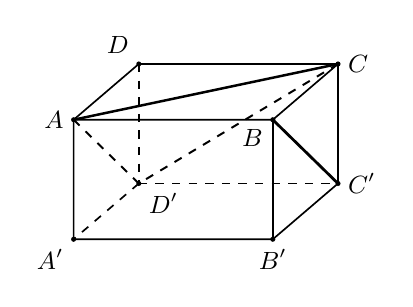
\begin{tikzpicture}[scale=0.92, line width=0.6pt, font=\small]

  \coordinate (A)  at (0,1.65);
  \coordinate (B)  at (2.75,1.65);
  \coordinate (C)  at (3.65,2.42);
  \coordinate (D)  at (0.90,2.42);
  \coordinate (Ap) at (0,0);
  \coordinate (Bp) at (2.75,0);
  \coordinate (Cp) at (3.65,0.77);
  \coordinate (Dp) at (0.90,0.77);

  % 可见棱
  \draw (A) -- (B) -- (C) -- (Cp) -- (Bp) -- (Ap) -- cycle;
  \draw (A) -- (D) -- (C);
  \draw (B) -- (Bp);

  % 不可见棱
  \draw[dashed] (D) -- (Dp);
  \draw[dashed] (Dp) -- (Cp);
  \draw[dashed] (Dp) -- (Ap);

  % 平面 D'AC 的边
  \draw[line width=0.9pt] (A) -- (C);
  \draw[dashed, line width=0.7pt] (A) -- (Dp) -- (C);

  % 直线 BC'
  \draw[line width=1.0pt] (B) -- (Cp);

  % 顶点
  \fill (A) circle (1pt) node[left] {$A$};
  \fill (B) circle (1pt) node[below left] {$B$};
  \fill (C) circle (1pt) node[right] {$C$};
  \fill (D) circle (1pt) node[above left] {$D$};
  \fill (Ap) circle (1pt) node[below left] {$A'$};
  \fill (Bp) circle (1pt) node[below] {$B'$};
  \fill (Cp) circle (1pt) node[right] {$C'$};
  \fill (Dp) circle (1pt) node[below right] {$D'$};

\end{tikzpicture}
\end{center}
\nopagebreak[4]
\Needspace{4\baselineskip}
\textbf{解析}
\Needspace{5\baselineskip}
以 $A$ 为原点，$\overrightarrow{AB}$、$\overrightarrow{AD}$、$\overrightarrow{AA'}$ 分别为 $x$、$y$、$z$ 轴正方向建立空间直角坐标系。由 $AB=2$，$AD=1$，$AA'=1$ 得
\nopagebreak[4]
\[A(0,0,0),\ B(2,0,0),\ D(0,1,0),\ A'(0,0,1),\]
\nopagebreak[4]
\[C(2,1,0),\ C'(2,1,1),\ D'(0,1,1).\]

\Needspace{5\baselineskip}
平面 $D'AC$ 经过 $A$、$C$、$D'$，取法向量
\nopagebreak[4]
\[\vec n=\overrightarrow{AC}\times\overrightarrow{AD'}
=(2,1,0)\times(0,1,1)
=(1,-2,2).\]
\Needspace{5\baselineskip}
直线 $BC'$ 的方向向量为
\nopagebreak[4]
\[\overrightarrow{BC'}=C'-B=(0,1,1).\]
\Needspace{5\baselineskip}
因为
\nopagebreak[4]
\[\vec n\cdot\overrightarrow{BC'}=1\cdot0+(-2)\cdot1+2\cdot1=0,\]
\Needspace{5\baselineskip}
所以 $BC'$ 的方向与平面 $D'AC$ 平行。又点 $B$ 不在平面 $D'AC$ 内（否则 $\vec n\cdot\overrightarrow{AB}=2\neq0$ 矛盾），故
\nopagebreak[4]
\[BC'\parallel\text{\text{平面} }D'AC.\]

\Needspace{5\baselineskip}
由于直线与平面平行，直线上任一点到平面的距离都相等。取点 $B$，距离为
\nopagebreak[4]
\[d=\frac{\left|\vec n\cdot\overrightarrow{AB}\right|}{|\vec n|}
=\frac{|(1,-2,2)\cdot(2,0,0)|}{\sqrt{1^2+(-2)^2+2^2}}
=\frac{2}{3}.\]
\Needspace{5\baselineskip}
故直线 $BC'$ 到平面 $D'AC$ 的距离为
\nopagebreak[4]
\[\frac23.\]

\gkanswer{答案：$\dfrac23$。以 $A$ 为原点建系，平面 $D'AC$ 的法向量可取 $(1,-2,2)$，$B$ 到该平面的距离为 $\dfrac{|(1,-2,2)\cdot(2,0,0)|}{3}=\dfrac23$。}

\end{answer}
\begin{answer}
\gksolhead{20}{}

\textbf{题目}：

甲厂以 $x$ 千克/小时的速度运输生产某种产品（生产条件要求 $1\leqslant x\leqslant10$），每一小时可获得利润是 $100\left(5x+1-\dfrac3x\right)$ 元。

（1） 要使生产该产品 $2$ 小时获得的利润不低于 $3000$ 元，求 $x$ 的取值范围；

（2） 要使生产 $900$ 千克该产品获得的利润最大，问：甲厂应该选取何种生产速度？并求最大利润。

\Needspace{4\baselineskip}
\textbf{解析}
\Needspace{5\baselineskip}
\textbf{（1）} 生产 $2$ 小时获得的利润为
\nopagebreak[4]
\[2\cdot100\left(5x+1-\frac3x\right)=200\left(5x+1-\frac3x\right).\]
\Needspace{5\baselineskip}
要求不低于 $3000$ 元：
\nopagebreak[4]
\[200\left(5x+1-\frac3x\right)\geqslant3000.\]
\Needspace{5\baselineskip}
两边除以 $200$：
\nopagebreak[4]
\[5x+1-\frac3x\geqslant15,\]
\Needspace{5\baselineskip}
即
\nopagebreak[4]
\[5x-14-\frac3x\geqslant0.\]
\Needspace{5\baselineskip}
因 $x>0$，两边乘以 $x$：
\nopagebreak[4]
\[5x^2-14x-3\geqslant0.\]
\Needspace{5\baselineskip}
因式分解：
\nopagebreak[4]
\[(5x+1)(x-3)\geqslant0.\]
\Needspace{5\baselineskip}
由于 $5x+1>0$，得 $x\geqslant3$。结合生产条件 $1\leqslant x\leqslant10$，有
\nopagebreak[4]
\[3\leqslant x\leqslant10.\]
即 $x$ 的取值范围为 $[3,10]$。

\Needspace{5\baselineskip}
\textbf{（2）} 生产 $900$ 千克所需时间为 $\dfrac{900}{x}$ 小时，总利润为
\nopagebreak[4]
\[P(x)=\frac{900}{x}\cdot100\left(5x+1-\frac3x\right)
=90000\left(5+\frac1x-\frac{3}{x^2}\right).\]
\Needspace{5\baselineskip}
令 $u=\dfrac1x$。由 $1\leqslant x\leqslant10$ 得 $u\in\left[\dfrac1{10},1\right]$，且
\nopagebreak[4]
\[P=90000\left(5+u-3u^2\right).\]
\Needspace{5\baselineskip}
二次函数 $5+u-3u^2$ 开口向下，对称轴为
\nopagebreak[4]
\[u=-\frac{1}{2\cdot(-3)}=\frac16.\]
\Needspace{5\baselineskip}
$\dfrac16\in\left[\dfrac1{10},1\right]$，故最大值在 $u=\dfrac16$ 处取得，即
\nopagebreak[4]
\[x=6.\]
\Needspace{5\baselineskip}
此时
\nopagebreak[4]
\[5+\frac16-3\cdot\frac1{36}
=5+\frac16-\frac1{12}
=5+\frac1{12}=\frac{61}{12},\]
\Needspace{5\baselineskip}
所以
\nopagebreak[4]
\[P_{\max}=90000\cdot\frac{61}{12}=7500\cdot61=457500.\]
端点比较：$x=1$ 时 $P=270000$，$x=10$ 时 $P=456300$，均小于 $457500$。故甲厂应选取 $6$ 千克/小时的生产速度，最大利润为 $457500$ 元。

\gkanswer{答案（1）：$[3,10]$。由 $200\left(5x+1-\dfrac3x\right)\geqslant3000$ 得 $x\geqslant3$，结合 $1\leqslant x\leqslant10$。}

\gkanswer{答案（2）：$x=6$ 千克/小时，最大利润 $457500$ 元。总利润 $90000\left(5+\dfrac1x-\dfrac{3}{x^2}\right)$，令 $u=\dfrac1x$，在 $u=\dfrac16$ 处取最大值。}

\end{answer}
\begin{answer}
\gksolhead{21}{}

\textbf{题目}：

已知函数 $f(x)=2\sin\omega x$，其中常数 $\omega>0$。

（1） 若 $y=f(x)$ 在 $\left[-\dfrac{\pi}{4},\dfrac{2\pi}{3}\right]$ 上单调递增，求 $\omega$ 的取值范围；

（2） 令 $\omega=2$，将函数 $y=f(x)$ 的图象向左平移 $\dfrac{\pi}{6}$ 个单位，再向上平移 $1$ 个单位，得到函数 $y=g(x)$ 的图象。区间 $[a,b]$（$a,b\in\mathbf R$ 且 $a<b$）满足：$y=g(x)$ 在 $[a,b]$ 上至少含有 $30$ 个零点，在所有满足上述条件的 $[a,b]$ 中，求 $b-a$ 的最小值。

\Needspace{4\baselineskip}
\textbf{解析}
\Needspace{5\baselineskip}
\textbf{（1）} 对 $f(x)=2\sin\omega x$（$\omega>0$），其单调递增区间为
\nopagebreak[4]
\[\left[-\frac{\pi}{2\omega}+\frac{2k\pi}{\omega},\ \frac{\pi}{2\omega}+\frac{2k\pi}{\omega}\right],\qquad k\in\mathbf Z.\]
\Needspace{5\baselineskip}
所给区间 $\left[-\dfrac{\pi}{4},\dfrac{2\pi}{3}\right]$ 含有 $0$，只能落在 $k=0$ 的单调递增区间内，即
\nopagebreak[4]
\[\left[-\frac{\pi}{4},\frac{2\pi}{3}\right]
\subseteq\left[-\frac{\pi}{2\omega},\frac{\pi}{2\omega}\right].\]
\Needspace{5\baselineskip}
于是
\nopagebreak[4]
\[-\frac{\pi}{4}\geqslant-\frac{\pi}{2\omega}
\Longrightarrow \omega\leqslant2,\]
\nopagebreak[4]
\[\frac{2\pi}{3}\leqslant\frac{\pi}{2\omega}
\Longrightarrow \omega\leqslant\frac34.\]
\Needspace{5\baselineskip}
两者取交集，并结合 $\omega>0$，得
\nopagebreak[4]
\[0<\omega\leqslant\frac34.\]

\Needspace{5\baselineskip}
\textbf{（2）} 当 $\omega=2$ 时，$f(x)=2\sin2x$。向左平移 $\dfrac{\pi}{6}$ 个单位得
\nopagebreak[4]
\[2\sin2\left(x+\frac{\pi}{6}\right)=2\sin\left(2x+\frac{\pi}{3}\right),\]
\Needspace{5\baselineskip}
再向上平移 $1$ 个单位得
\nopagebreak[4]
\[g(x)=2\sin\left(2x+\frac{\pi}{3}\right)+1.\]
\Needspace{5\baselineskip}
零点满足
\nopagebreak[4]
\[\sin\left(2x+\frac{\pi}{3}\right)=-\frac12.\]
\Needspace{5\baselineskip}
于是
\nopagebreak[4]
\[2x+\frac{\pi}{3}=-\frac{\pi}{6}+2k\pi
\quad\text{\text{或}}\quad
2x+\frac{\pi}{3}=\frac{7\pi}{6}+2k\pi,\]
\Needspace{5\baselineskip}
即
\nopagebreak[4]
\[x=-\frac{\pi}{4}+k\pi
\quad\text{\text{或}}\quad
x=\frac{5\pi}{12}+k\pi,\qquad k\in\mathbf Z.\]
\Needspace{5\baselineskip}
把零点按从小到大排列：
\nopagebreak[4]
\[\cdots,\ -\frac{\pi}{4},\ \frac{5\pi}{12},\ \frac{3\pi}{4},\ \frac{17\pi}{12},\ \cdots\]
\Needspace{5\baselineskip}
相邻零点的间距交替为
\nopagebreak[4]
\[\frac{5\pi}{12}-\left(-\frac{\pi}{4}\right)=\frac{2\pi}{3},
\qquad
\frac{3\pi}{4}-\frac{5\pi}{12}=\frac{\pi}{3}.\]

\Needspace{5\baselineskip}
若区间 $[a,b]$ 含有至少 $30$ 个零点，则其中必可取出 $30$ 个连续零点。这 $30$ 个零点之间有 $29$ 个间隔。由于间隔按 $\dfrac{2\pi}{3}$ 与 $\dfrac{\pi}{3}$ 交替，$29$ 个连续间隔中必有一种出现 $15$ 次、另一种出现 $14$ 次。其和的最小值为
\nopagebreak[4]
\[15\cdot\frac{\pi}{3}+14\cdot\frac{2\pi}{3}
=5\pi+\frac{28\pi}{3}
=\frac{43\pi}{3}.\]
\Needspace{5\baselineskip}
该值可以取到：从零点 $\dfrac{5\pi}{12}$ 开始，向后数到第 $30$ 个零点，所得区间恰好跨过 $15$ 个 $\dfrac{\pi}{3}$ 间隔和 $14$ 个 $\dfrac{2\pi}{3}$ 间隔。因此
\nopagebreak[4]
\[(b-a)_{\min}=\frac{43\pi}{3}.\]

\gkanswer{答案（1）：$\left(0,\dfrac34\right]$。需 $\left[-\dfrac{\pi}{4},\dfrac{2\pi}{3}\right]\subseteq\left[-\dfrac{\pi}{2\omega},\dfrac{\pi}{2\omega}\right]$，故 $\omega\leqslant\dfrac34$。}

\gkanswer{答案（2）：$\dfrac{43\pi}{3}$。零点为 $x=-\dfrac{\pi}{4}+k\pi$ 或 $x=\dfrac{5\pi}{12}+k\pi$，相邻零点间距交替为 $\dfrac{2\pi}{3}$ 与 $\dfrac{\pi}{3}$；含 $30$ 个零点的最短区间跨 $29$ 个间隔，取 $15$ 个 $\dfrac{\pi}{3}$ 与 $14$ 个 $\dfrac{2\pi}{3}$ 时最小。}

\end{answer}
\begin{answer}
\gksolhead{22}{}

\textbf{题目}：

如图，已知双曲线 $C_1:\dfrac{x^2}{2}-y^2=1$，曲线 $C_2:|y|=|x|+1$。$P$ 是平面内一点，若存在过点 $P$ 的直线与 $C_1$、$C_2$ 都有公共点，则称 $P$ 为“$C_1-C_2$ 型点”。
\nopagebreak[4]
\begin{center}% ============================================================
% f2013_shanghai_science_q22_hyperbola.tex
% 2013 上海卷（理科）第 22 题 双曲线 C1 与折线 C2（TikZ 矢量重绘）
% 曲线：C1: x^2/2 - y^2 = 1（两支，顶点在 (±sqrt2, 0)）；
%       C2: |y| = |x| + 1（两条折线，顶点分别在 (0,1)、(0,-1)，四臂斜率 ±1）。
% 坐标轴等比例，便于看出 C1 渐近线 y = ±x/sqrt2 与 C2 四臂的方向差别。
% ============================================================
\begin{tikzpicture}[
  x=1.1cm, y=1.1cm,
  every node/.style={font=\small, inner sep=1pt},
  line/.style={line width=0.6pt},
  axis/.style={line width=0.5pt, -{Stealth[length=2.2mm,width=1.6mm]}},
]

  % 坐标轴
  \draw[axis] (-3.25,0) -- (3.45,0);
  \draw[axis] (0,-2.85) -- (0,3.05);

  % C1 的左右两支：x = ±sqrt(2(1+t^2)), y = t
  \draw[line, domain=-2.03:2.03, samples=120, smooth, variable=\t]
    plot ({sqrt(2*(1+\t*\t))}, {\t});
  \draw[line, domain=-2.03:2.03, samples=120, smooth, variable=\t]
    plot ({-sqrt(2*(1+\t*\t))}, {\t});

  % C2 的两条折线：|y| = |x| + 1
  \draw[line] (-1.92,2.92) -- (0,1) -- (1.92,2.92);
  \draw[line] (-1.92,-2.92) -- (0,-1) -- (1.92,-2.92);

  % 原点与轴标签
  \node at (-0.34,-0.38) {$O$};
  \node at (3.62,-0.24) {$x$};
  \node at (-0.26,3.22) {$y$};

\end{tikzpicture}
\end{center}
\nopagebreak[4]
（1） 在正确证明 $C_1$ 的左焦点是“$C_1-C_2$ 型点”时，要使用一条过该焦点的直线，试写出一条这样的直线的方程（不要求验证）；

（2） 设直线 $y=kx$ 与 $C_2$ 有公共点，求证 $|k|>1$，进而证明原点不是“$C_1-C_2$ 型点”；

（3） 求证：圆 $x^2+y^2=\dfrac12$ 内的点都不是“$C_1-C_2$ 型点”。

\Needspace{4\baselineskip}
\textbf{解析}
\Needspace{5\baselineskip}
\textbf{（1）} 双曲线 $C_1:\dfrac{x^2}{2}-y^2=1$ 中 $a^2=2$，$b^2=1$，故
\nopagebreak[4]
\[c^2=a^2+b^2=3,\qquad c=\sqrt3.\]
\Needspace{5\baselineskip}
左焦点为 $F(-\sqrt3,0)$。取过 $F$ 的竖直线
\nopagebreak[4]
\[x=-\sqrt3.\]
\Needspace{5\baselineskip}
它与 $C_1$ 的交点满足
\nopagebreak[4]
\[\frac32-y^2=1\Longrightarrow y^2=\frac12\Longrightarrow y=\pm\frac{\sqrt2}{2},\]
\Needspace{5\baselineskip}
有公共点；它与 $C_2$ 的交点满足
\nopagebreak[4]
\[|y|=|-\sqrt3|+1=\sqrt3+1,\]
也有公共点。故 $x=-\sqrt3$ 即为所求（答案不唯一）。

\Needspace{5\baselineskip}
\textbf{（2）} 设直线 $y=kx$ 与 $C_2$ 有公共点 $(x,y)$。若 $x=0$，则 $y=0$，但 $C_2$ 上 $x=0$ 时 $|y|=1$，矛盾，故 $x\neq0$。代入 $|y|=|x|+1$：
\nopagebreak[4]
\[|k|\,|x|=|x|+1
\Longrightarrow |x|\left(|k|-1\right)=1.\]
\Needspace{5\baselineskip}
因 $|x|>0$，必须
\nopagebreak[4]
\[|k|-1>0\Longrightarrow |k|>1.\]

再证原点不是“$C_1-C_2$ 型点”。过原点的直线分两类。

\Needspace{5\baselineskip}
若直线为 $y=kx$ 且与 $C_2$ 有公共点，由上一段得 $|k|>1$。代入 $C_1$：
\nopagebreak[4]
\[\frac{x^2}{2}-k^2x^2=1
\Longrightarrow x^2\left(\frac12-k^2\right)=1.\]
因 $k^2>1>\dfrac12$，左端系数为负，而右端为正，方程无实根，故该直线与 $C_1$ 无公共点。

若直线为 $y$ 轴 $x=0$，代入 $C_1$ 得 $-y^2=1$，无实根，与 $C_1$ 无公共点。

所以不存在过原点且与 $C_1$、$C_2$ 都有公共点的直线，原点不是“$C_1-C_2$ 型点”。

\Needspace{5\baselineskip}
\textbf{（3）} 设 $P(x_0,y_0)$ 满足
\nopagebreak[4]
\[x_0^2+y_0^2<\frac12,\]
$l$ 是过 $P$ 的任意直线。证明 $l$ 不可能同时与 $C_1$、$C_2$ 有公共点。

\Needspace{5\baselineskip}
若 $l$ 的斜率不存在，则 $l:x=x_0$。由
\nopagebreak[4]
\[|x_0|\leqslant\sqrt{x_0^2+y_0^2}<\frac1{\sqrt2}<\sqrt2,\]
\Needspace{5\baselineskip}
得 $\dfrac{x_0^2}{2}<1$。而 $C_1$ 上的点满足
\nopagebreak[4]
\[\frac{x^2}{2}=1+y^2\geqslant1,\]
所以 $l$ 与 $C_1$ 无公共点。

\Needspace{5\baselineskip}
以下设 $l:y=kx+m$。原点 $O$ 到 $l$ 的距离为 $\dfrac{|m|}{\sqrt{1+k^2}}$。因 $l$ 过 $P$，该距离不超过 $|OP|$，故
\nopagebreak[4]
\[\frac{|m|}{\sqrt{1+k^2}}\leqslant|OP|<\frac1{\sqrt2}
\Longrightarrow m^2<\frac{1+k^2}{2}. \tag{*}\]

\Needspace{5\baselineskip}
若 $|k|\leqslant1$，由 (*) 得
\nopagebreak[4]
\[m^2<\frac{1+k^2}{2}\leqslant1,\]
\Needspace{5\baselineskip}
即 $|m|<1$。对 $l$ 上任意点 $(x,kx+m)$，
\nopagebreak[4]
\[|y|=|kx+m|\leqslant|k|\,|x|+|m|<|x|+1,\]
故 $l$ 上不存在满足 $|y|=|x|+1$ 的点，$l$ 与 $C_2$ 无公共点。

\Needspace{5\baselineskip}
若 $|k|>1$，把 $y=kx+m$ 代入 $C_1$：
\nopagebreak[4]
\[\frac{x^2}{2}-(kx+m)^2=1.\]
\Needspace{5\baselineskip}
两边乘以 $2$ 并整理：
\nopagebreak[4]
\[\left(1-2k^2\right)x^2-4kmx-2\left(m^2+1\right)=0.\]
\Needspace{5\baselineskip}
其判别式为
\nopagebreak[4]
\[\begin{aligned}
\Delta
&=16k^2m^2+8\left(1-2k^2\right)\left(m^2+1\right)\\
&=8\left(m^2+1-2k^2\right).
\end{aligned}\]
\Needspace{5\baselineskip}
由 (*) 得
\nopagebreak[4]
\[m^2+1-2k^2<\frac{1+k^2}{2}+1-2k^2
=\frac{3-3k^2}{2}<0,\]
故 $\Delta<0$，方程无实根，$l$ 与 $C_1$ 无公共点。

综上，过圆 $x^2+y^2=\dfrac12$ 内任一点的直线都不可能同时与 $C_1$、$C_2$ 有公共点，即圆内的点都不是“$C_1-C_2$ 型点”。

\gkanswer{答案（1）：$x=-\sqrt3$（答案不唯一）。左焦点为 $(-\sqrt3,0)$，该竖直线与 $C_1$、$C_2$ 均有公共点。}

\gkanswer{答案（2）：证明见解析。由 $|k||x|=|x|+1$ 得 $|k|>1$；过原点的直线若与 $C_2$ 有公共点则 $|k|>1$，此时代入 $C_1$ 无实根；$y$ 轴也与 $C_1$ 无公共点。}

\gkanswer{答案（3）：证明见解析。圆内点 $P$ 满足 $|OP|<\dfrac1{\sqrt2}$；过 $P$ 的直线到原点距离小于 $\dfrac1{\sqrt2}$，再按 $|k|\leqslant1$ 与 $|k|>1$ 分别证明它不能同时与 $C_1$、$C_2$ 相交。}

\end{answer}
\begin{answer}
\gksolhead{23}{}

\textbf{题目}：

给定常数 $c>0$，定义函数 $f(x)=2|x+c+4|-|x+c|$，数列 $a_1,a_2,a_3,\cdots$ 满足 $a_{n+1}=f(a_n)$，$n\in\mathbf N^*$。

（1） 若 $a_1=-c-2$，求 $a_2$ 及 $a_3$；

（2） 求证：对任意 $n\in\mathbf N^*$，$a_{n+1}-a_n\geqslant c$；

（3） 是否存在 $a_1$，使得 $a_1,a_2,\cdots,a_n,\cdots$ 成等差数列？若存在，求出所有这样的 $a_1$；若不存在，说明理由。

\Needspace{4\baselineskip}
\textbf{解析}
\Needspace{5\baselineskip}
令 $t=x+c$，则
\nopagebreak[4]
\[f(x)=2|t+4|-|t|.\]
按 $t$ 的符号分段：

\begin{itemize}
\item 当 $t\geqslant0$，即 $x\geqslant-c$ 时，
\end{itemize}
\nopagebreak[4]
\[f(x)=2(t+4)-t=t+8=x+c+8;\]
\begin{itemize}
\item 当 $-4\leqslant t<0$，即 $-c-4\leqslant x<-c$ 时，
\end{itemize}
\nopagebreak[4]
\[f(x)=2(t+4)+t=3t+8=3x+3c+8;\]
\begin{itemize}
\item 当 $t<-4$，即 $x<-c-4$ 时，
\end{itemize}
\nopagebreak[4]
\[f(x)=-2(t+4)+t=-t-8=-x-c-8.\]

\Needspace{5\baselineskip}
\textbf{（1）} 由 $a_1=-c-2$，得
\nopagebreak[4]
\[a_1+c=-2\in[-4,0),\]
\Needspace{5\baselineskip}
故 $a_1$ 落在中间段：
\nopagebreak[4]
\[a_2=3(-c-2)+3c+8=-3c-6+3c+8=2.\]
\Needspace{5\baselineskip}
又 $a_2=2>-c$，落在 $x\geqslant-c$ 段：
\nopagebreak[4]
\[a_3=a_2+c+8=2+c+8=c+10.\]
\Needspace{5\baselineskip}
所以
\nopagebreak[4]
\[a_2=2,\qquad a_3=c+10.\]

\textbf{（2）} 分三段计算 $f(x)-x$。

\Needspace{5\baselineskip}
当 $x\geqslant-c$ 时，
\nopagebreak[4]
\[f(x)-x=(x+c+8)-x=c+8\geqslant c.\]
\Needspace{5\baselineskip}
当 $-c-4\leqslant x<-c$ 时，
\nopagebreak[4]
\[f(x)-x=(3x+3c+8)-x=2x+3c+8.\]
\Needspace{5\baselineskip}
因 $x\geqslant-c-4$，
\nopagebreak[4]
\[2x+3c+8\geqslant2(-c-4)+3c+8=c.\]
\Needspace{5\baselineskip}
当 $x<-c-4$ 时，
\nopagebreak[4]
\[f(x)-x=(-x-c-8)-x=-2x-c-8.\]
\Needspace{5\baselineskip}
因 $x<-c-4$，
\nopagebreak[4]
\[-2x-c-8>2(c+4)-c-8=c.\]
\Needspace{5\baselineskip}
综上，对一切实数 $x$，
\nopagebreak[4]
\[f(x)-x\geqslant c.\]
\Needspace{5\baselineskip}
取 $x=a_n$，即得
\nopagebreak[4]
\[a_{n+1}-a_n=f(a_n)-a_n\geqslant c,\qquad n\in\mathbf N^*.\]

\Needspace{5\baselineskip}
\textbf{（3）} 假设 $\{a_n\}$ 为等差数列，公差为 $d$。由（2）知
\nopagebreak[4]
\[d=a_{n+1}-a_n\geqslant c>0,\]
\Needspace{5\baselineskip}
故 $a_n\to+\infty$。于是存在 $N$，当 $n\geqslant N$ 时 $a_n\geqslant-c$，此时
\nopagebreak[4]
\[a_{n+1}=f(a_n)=a_n+c+8,\]
\Needspace{5\baselineskip}
从而
\nopagebreak[4]
\[d=a_{n+1}-a_n=c+8.\]
\Needspace{5\baselineskip}
因此对每个 $n$，都必须有
\nopagebreak[4]
\[f(a_n)-a_n=c+8.\]

\Needspace{5\baselineskip}
先看 $a_1\geqslant-c$ 的情形：此时
\nopagebreak[4]
\[a_{n+1}=f(a_n)=a_n+c+8,\]
所以 $\{a_n\}$ 是以 $c+8$ 为公差的等差数列。故所有 $a_1\geqslant-c$ 都满足要求。

\Needspace{5\baselineskip}
再看 $a_1<-c$ 的情形。因公差 $d=c+8$，必须有
\nopagebreak[4]
\[f(a_1)-a_1=c+8.\]
\Needspace{5\baselineskip}
若 $-c-4\leqslant a_1<-c$，则
\nopagebreak[4]
\[2a_1+3c+8=c+8\Longrightarrow a_1=-c,\]
与 $a_1<-c$ 矛盾。
\Needspace{5\baselineskip}
若 $a_1<-c-4$，则
\nopagebreak[4]
\[-2a_1-c-8=c+8\Longrightarrow a_1=-c-8.\]
\Needspace{5\baselineskip}
检验 $a_1=-c-8$：
\nopagebreak[4]
\[a_1+c=-8,\qquad a_2=2|-4|-|-8|=8-8=0,\]
\nopagebreak[4]
\[a_2-a_1=0-(-c-8)=c+8,\]
且 $a_2=0\geqslant-c$，此后每项都按 $a_{n+1}=a_n+c+8$ 递增，故确为等差数列。

\Needspace{5\baselineskip}
综上，存在这样的 $a_1$，全部为
\nopagebreak[4]
\[a_1\geqslant-c\quad\text{\text{或}}\quad a_1=-c-8.\]

\gkanswer{答案（1）：$a_2=2$，$a_3=c+10$。$a_1+c=-2$ 落在中间段，$a_2=2$ 落在 $x\geqslant-c$ 段。}

\gkanswer{答案（2）：证明见解析。分段计算得 $f(x)-x\geqslant c$ 对一切 $x$ 成立。}

\gkanswer{答案（3）：存在，$a_1\geqslant-c$ 或 $a_1=-c-8$。等差数列公差 $d\geqslant c>0$，项最终进入 $x\geqslant-c$ 段，故 $d=c+8$；再逐项检验首项即可。}

\end{answer}